\chapter{Project Design} 
% Main chapter title

\label{Chapter3} 
%Call reference to this2 chapter use \ref{ChapterX}

\lhead{Chapter 3. \emph{Project Design}} 
% Change X to a consecutive number; this is for the header on each page - perhaps a shortened title

\doublespacing
% LINE FORMATTING

%\clearpage
%\pagebreak

% MAIN SECTION =============================

\section{Phase 1}


\subsection{Introduction}
The primary focus of Phase 1 is implement prototype to prove theoretical concepts of the domain to research in this project. Requirements are listed as follow:

\begin{enumerate}[topsep=0pt,itemsep=-1ex,partopsep=1ex,parsep=1.5ex]

\item To acquire free large data set for big data processing.
\item To ensure data set acquired from the website are free, consent and clean with Devil Advocation Test. 
\item A program will be implemented in RUST and Go programming language as a proof-of-concept (POC) that CSV raw data is capable of importing into PostgreSQL database.
\item A program will be implemented with Go programming language as POC that PostgreSQL database transaction can be sequential and concurrent.
\item A program will be implemented with Go programming language as POC that reading CSV files can be sequential and concurrent.
\item To ease the debugging and troubleshooting on concurrent and distributed development environment, LTTng tracing network and Eclipse Trace Compass will be installed to obtain a reading and outputs traces via Common Trace File (CTF) binary format. 

\end{enumerate}

\pagebreak

\subsection{Data Collection}

The project is required to work with large data sets to utilize infrastructure and processing power of GO and RUST concurrent programming language. Data collection is conducted to identify of company recruitment preferences on higher education graduates of different subjects in the UK with basic company and LEO datasets. Data collected is required to be clean and able to solve interesting problem or question. 

The characteristic of free, consent and licensed data sets acquired from UK government website provider (data.gov.uk) are as follow:

\begin{table}[H]
	\resizebox{\textwidth}{!}{%
	\begin{tabulary}{1.0\textwidth}{|L|L|L|L|L|L}
		\hline
		{\bf No} & {\bf Name of Datasets}  						& {\bf Column } & {\bf Rows} & {\bf Size}	\\ \hline
		1.       & Longitudinal Educations Outcomes (LEO)       &  21          & 32706       & 1.8   GB		\\ \hline
		2.       & Basic Company Profile (Company)              &  55          & 3595702     & 667.5 MB		\\ \hline
		3.       & National Statistics Postcode Lookup (NSPL)   &  35          & 1754882     & 4.2	 MB		\\ \hline
	\end{tabulary}}
	\caption{Result of Golang programming on process CSV raw data}
\end{table}

The file format of all large dataset obtained are Comma Separated Values (CSV) format which the information is organized with one record as one line and each field is separated by comma (,). CSV format is used for data processing in this project because it is human readable and simple to be parse. It can be handle using PostgreSQL database and retrievable by programs. 

\pagebreak

\subsubsection{Longitudinal Education Outcomes (LEO) dataset }

The data set focus on employment and earnings outcome of Bachelor’s Degree graduate in Great Britain after five years. It contains information about students include personal characteristics, education or qualification achieved, employment and income earnings.  The data dictionary of longitudinal education outcome is created and placed in Appendix I.1.1.

\subsubsection{Basic Company dataset}

The data set possesses up-to-date basic companies information on UK register. It contains company names, annual returns filing dates, location details, account and basic information about mortgage and business changes. The data dictionary of basic company dataset is created and placed in Appendix I.1.2.

\subsubsection{National Statistics Postcode Lookup (NSPL) dataset}

\begin{figure}[H]
	\centering
	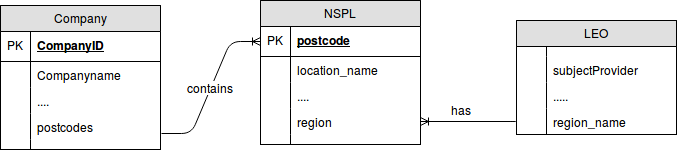
\includegraphics[width=0.9\textwidth]{Figure/erd-data.png}
	\rule{35em}{0.5pt}
	\caption[Entity Relationship Diagram]{Entity Relationship Diagram}
\end{figure}

As postcode data for every location on earth is unique. Company data sets possess \textbf{postcode} field in the business address, but LEO dataset do not have the \textbf{postcode} field which leads to difficulty of defining a relationship between these two datasets. Figure above show NSPL dataset serves as a linker to map \textbf{region} column from LEO data to link with \textbf{postcode} column found in company datasets.

The data set possesses current postcode for the United Kingdom. It contains information relates postcode number, location, country name, parliamentary constitution, electoral and other geographical details. The data dictionary of National Statistics Postcode Lookup (NSPL) dataset is created and placed in Appendix I.1.3.



\subsection{Data Validation}

\begin{figure}[H]
	\centering
	\includegraphics[width=1.0\textwidth]{FYP2/Chapter3/FYP2-data-validation-flowchart.png}
	\rule{35em}{0.7pt}
	\caption[Data Validation Procedure Flowchart]{Data Validation Procedure Flowchart}
\end{figure}

Data validation is conducted to inspect the quality dimension of data sources acquire in Data Collection (Section 3.1.2) to prevent corruption, inconsistency and conflicts during importing, using and processing. It is performed to ensure the data acquired are clean and in excellent quality. 

The important steps taken on validation of data are shown in Figure 3.5. The \textbf{completeness} of datasets will be examine to assures the characteristic of data fulfill Comma Separate Values (CSV) standard and requirement. The common test performed during data completeness check are using aggregate functions such as max, min or counts. \cite{data-completeness-check}

Furthermore, the \textbf{validity} of data types in each columns are measured to prevent incompatible data types during Data Importation, Object Relational Mapping (ORM) and Data Migration. The types of data stored in each columns of obtained datasets shall be identify to describe suitable data type for Database Definition Language (DDL) during database table creation. As an example, the alphanumeric and text field are usually defined as VARCHAR and field contains only number will be declared as INTEGER.  

In addition, the \textbf{uniqueness} of records will be verify to discover wasteful and duplication of data. The data redundancy indicates same piece of data are exist in multiple place. \cite{data-redundancy-definition} This condition will results in waste of space, data inconsistency and violates data integrity. If the duplication of data is discovered, database normalization will be performed to eliminate the duplication of records. 

Last but not least, the \textbf{consistency} of data will be analyze to ensure datasets obtained are conform to specific standards and meet requirements. The data consistency check shall be performed during data preparation to inspect discover missing, corrupted or invalid data in record. The conformity and consistency of data in specific column should be handled in wariness to prevent affect the outcomes and efficiency of data processing. If the data is found inconsistent, Data Cleaning and Data Importation will be conducted to fix the defects discovered in the datasets. 

\subsection{Performance Benchmarking}

To conduct a comparison between Go and RUST language, benchmarking plays an important role to achieve fairness in compare performance and expressive power of language.

The component that are benchmarked are listed below:  

\begin{enumerate}[topsep=0pt,itemsep=-1ex,partopsep=1ex,parsep=1.5ex]
	
	\item \textbf{SQL Queries run on program. } Go and Rust program execute the same amount of database retrieval query to achieve the fairness of comparison.
	\newline
	\item \textbf{Table configurations.} The space of table of this project should be same for Go and Rust program to test the performance. 
	\newline
	\item \textbf{Hardware configurations. } Both Go and Rust program are required to run on same hardware configuration to achieve fairness of comparison on performance.
	\newline
	
\end{enumerate}

\pagebreak

\subsection{Database Retrieval Program}

\subsubsection{Phase 1 System Context Diagram}

\begin{figure}[H]
	\centering
	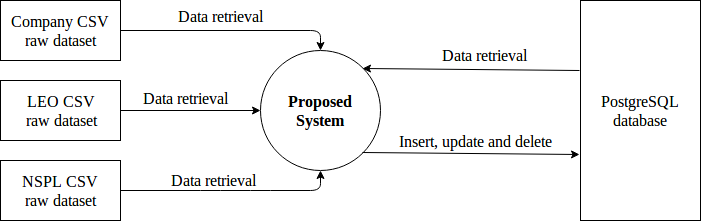
\includegraphics[width=0.9\textwidth]{Figure/fyp-context.png}
	\rule{35em}{0.5pt}
	\caption[Phase 1 System Context Diagram]{Phase 1 System Context Diagram}
\end{figure}

System context diagram provide high level view that defines relationship between proposed system with external entities. The proposed system is written in Go and Rust programming language with sequential and concurrent computing. The system shall process raw dataset stores in different nodes and dataset stores in PostgreSQL database. Moreover, the system should process data from raw CSV dataset and PostgreSQL database in sequential and concurrent manner. 

\subsubsection{Phase 1 Block Diagram}

\begin{figure}[H]
	\centering
	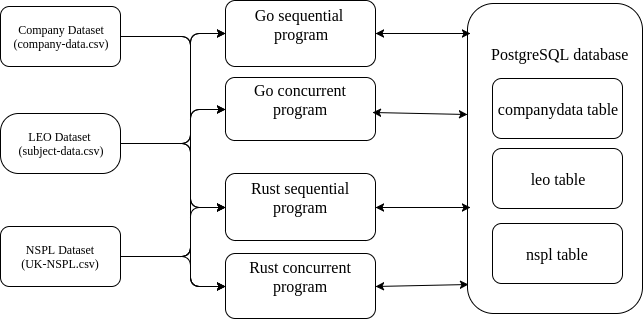
\includegraphics[width=0.9\textwidth]{Figure/block-diagram.png}
	\rule{35em}{0.5pt}
	\caption[Phase 1 Block Diagram]{Phase 1 Block Diagram}
\end{figure}

The block diagram provides a high-level overview of importation CSV into PostgreSQL with Go and Rust program. The large dataset store is store in different nodes with CSV format. Data stores in PostgreSQL database and raw CSV data at different nodes will be processed by Go and Rust program with sequential and concurrent manner. The database table is created with query in the terminal before Go and Rust program is executed.

\subsection{PostgreSQL Database Retrieval with Go and Rust program}

\subsubsection{Phase 1 Sequential Program Flowchart}

\begin{figure}[H]
	\centering
	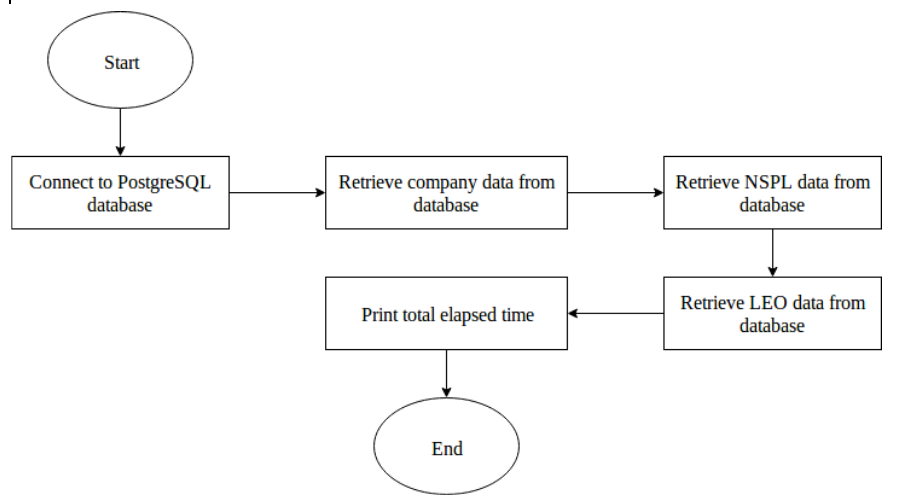
\includegraphics[width=0.9\textwidth]{Figure/postgres-data-sequential.png}
	\rule{35em}{0.5pt}
	\caption[Phase 1 Sequential program flowchart]{Phase 1 Sequential program flowchart}
\end{figure}

The flowchart provides a high-level view of concurrent manner during data retrieval in PostgreSQL with Go and Rust program. The program first establishes connection with PostgreSQL database with a connection string. Afterwards, it will retrieve a different set of data from various database table concurrently. The total elapsed time for entire program execution will be print.

\subsubsection{Phase 1 Concurrent Program Flowchart}

\begin{figure}[H]
	\centering
	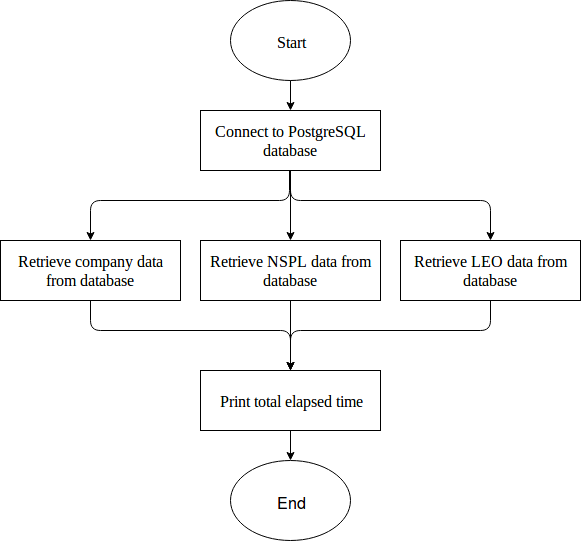
\includegraphics[width=0.9\textwidth]{Figure/postgres-data-concurrent.png}
	\rule{35em}{0.5pt}
	\caption[Phase 1 Concurrent program flowchart]{Phase 1 Concurrent program flowchart}
\end{figure}

The flowchart provides a high-level view on concurrent manner during data retrieval in PostgreSQL with Go and Rust program. The program first establish connection with PostgreSQL database with connection string. Afterwards, it will retrieve different set of data from different database table in concurrent manner. The total elapsed time for entire program execution will be print. 

\subsection{Raw CSV Data Retrieval with Go and Rust program}

\subsubsection{Phase 1 Sequential Program Flowchart}

\begin{figure}[H]
	\centering
	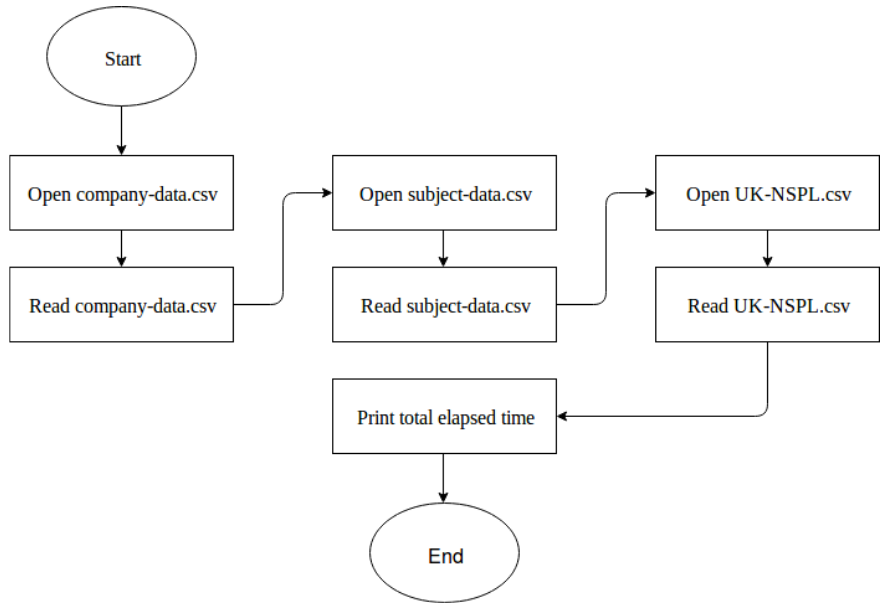
\includegraphics[width=0.9\textwidth]{Figure/seq-read-csv.png}
	\rule{35em}{0.5pt}
	\caption[Phase 1 Sequential program flowchart]{Phase 1 Sequential program flowchart}
\end{figure}

The flowchart provides a high-level view on sequential manner on reading CSV file with Go and Rust program. The program will open csv file and read containing data concurrently. The total elapsed time for entire program execution will be print.

\subsubsection{Phase 1 Concurrent Program Flowchart}

\begin{figure}[H]
	\centering
	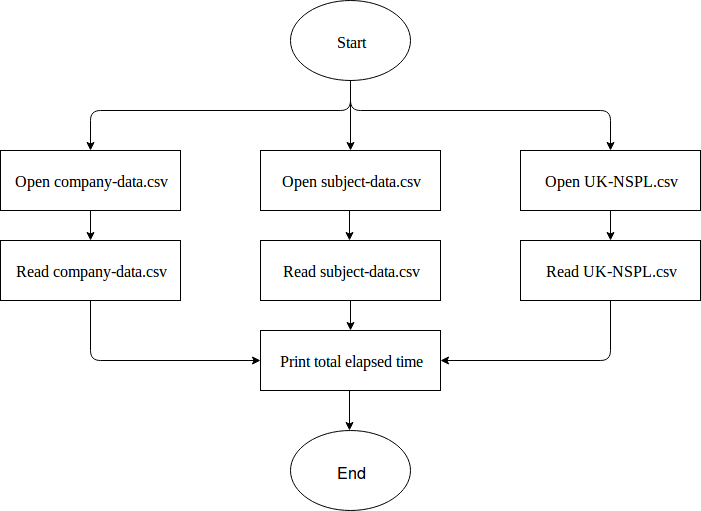
\includegraphics[width=0.9\textwidth]{Figure/concurrent-read-csv.png}
	\rule{35em}{0.5pt}
	\caption[Phase 1 Concurrent program flowchart]{Phase 1 Concurrent program flowchart}
\end{figure}

The flowchart provides a high-level view on concurrent manner on reading CSV file with Go and Rust program. The program will open csv file and read containing data in particular order of sequence. The total elapsed time for entire program execution will be print. 

\subsection{Proof of Concept in Phase 1}

\subsubsection{Phase 1 Deployment Diagram}

\begin{figure}[H]
	\centering
	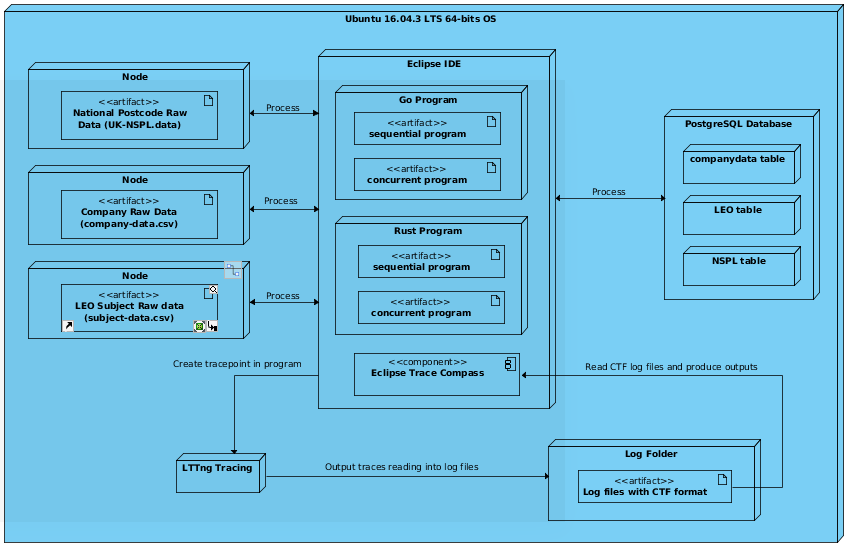
\includegraphics[width=1.0\textwidth]{Figure/dd-poc.png}
	\rule{35em}{0.5pt}
	\caption[Phase 1 Deployment Diagram]{Phase 1 Deployment Diagram}
\end{figure}

The deployment diagram describes the proof of concept of phase 1 in specification level and overall architecture of the project. Three database table is created in PostgreSQL database prepare to be processed. Simultaneously, three large data sets are stored in different nodes await to be process or retrieved. The Go and Rust program are written in sequentially and concurrently to process data from CSV file or PostgreSQL database system.

\section{Phase 2}

\subsection{Introduction}

Figure below shows Data Processing Cycle to provide an overview of activities carried out to process big data with the utilization of concurrent programming language and Structure Query Language (SQL).

\begin{figure}[H]
	\centering
	\includegraphics[width=1.0\textwidth]{FYP2/Chapter3/FYP2-data-process-cycle-flowchart.png}
	\rule{35em}{0.5pt}
	\caption[Data Process Cycle]{Data Process Cycle}
\end{figure} 

In Phase 2, we have established an extensive understanding on concurrent language characteristic by utilized the languages' feature on each activity in data processing cycle. The requirement as listed as follow: 

\begin{enumerate}[topsep=0pt,itemsep=-1ex,partopsep=1ex,parsep=1.5ex]
	
	\item Data encoding will be conducted with stream editor to convert dirty data into consistent format.
	\item Data transformation will be conducted to extracted data from CSV file and import into PostgreSQL database for data handling.
	\item Database normalization will be perform to eliminate data redundancy and improve data integrity.
	\item The structure of database schema and object (user and tables) will be created with scripts written in Data Definition Language (DDL) of PL/pgSQL (Procecural Language/PostgreSQL). 
	\item A \textbf{sequential} and \textbf{concurrent} program will be implemented with Go programming language as an Object Relational Mapping (O/R mapping tool) to convert raw data from CSV data sources into object model, the performance execution will be recorded and compared. 
	\item A \textbf{sequential} and \textbf{concurrent} program will be implemented with Go programming language as ORM tool to convert data retrieve from PostgreSQL database into object model, the performance execution will be recorded and compared.  
	\item A \textbf{sequential} and \textbf{concurrent} program will be implemented with Rust programming language as ORM tool to convert raw data from CSV data sources into object model, the performance execution will be recorded and compared. 
	\item A \textbf{sequential} and \textbf{concurrent} program will be implemented with Rust programming language as ORM tool to convert data retrieve from PostgreSQL database into object model, the performance execution will be recorded and compared.
	\item Data cleaning will be performed on CSV raw data to eliminate missing records and standardize the fields in common format. 
	\item Database tuning will be conducted to configure PostgreSQL database's environment for performance optimization on processing large-scale data and handling workloads. 
	\item A \textbf{sequential} and \textbf{concurrent} program will be implemented with Go programming language as data importation tool to export Company raw data from CSV data sources and import into PostgreSQL database. 
	\item Query tuning will be conducted to increase query execution performance on data processing. 
	\item Several \textbf{concurrent} program will be implemented with Go programming language as data migration tool to transfer company and NSPL data from legacy storage into normalized table within PostgreSQL database. 
	\item Data Manipulation Language (DML) scripts will be written with PL/pgSQL to transfer raw data from legacy storage into normalized table within PostgreSQL database.  
	\item Data verification will be conducted with UNIX command line to check the accuracy and consistency of database records after the data migration is complete. 
	
\end{enumerate}

\section{Data Encoding}

\subsection{Phase 2 Architecture Diagram}

\begin{figure}[H]
	\centering
	\includegraphics[width=1.0\textwidth]{FYP2/Chapter3/FYP2-data-encoding.png}
	\rule{35em}{0.5pt}
	\caption[Data Encoding Architecture Diagram]{Data Encoding Architecture Diagram}
\end{figure} 

Data encoding is a conversion of records or fields into specialized format for efficient transformation, importation and migration. \cite{data-encoding-definition} Figure 3.14 shows an architecture diagram that describe a high-level view of data encoding flow. The sed stream editor provide powerful feature to perform editing operations coming from a file to remove inconsistency data. \cite{sed-usage} 

The stream editor allow developer to make editing decisions by calling the commands on terminal. It consumes the dirty raw data as input file and perform text substitution line-by-line based on the text patterns of regular expressions provided in the commands. Ultimately, the encoded file will be output and store into the same directory. 

\section{Data Transformation}

\subsection{Phase 2 Architectural Diagram}

\begin{figure}[H]
	\centering
	\includegraphics[width=1.0\textwidth]{FYP2/Chapter3/FYP2-data-transformation-arc.png}
	\rule{35em}{0.5pt}
	\caption[Data Transformation Architectural Diagram]{Data Transformation Architectural Diagram}
\end{figure} 


Data transformation is the process of converting one format to another by extracting from source application into data warehouse. \cite{data-transformation-definition} 

Figure 3.15 shows the architectural diagram of data transformation process in this project. After the data inconsistency is eliminated with data encoding (performed in Section 3.3), the data in CSV format is extracted and import into PostgreSQL database with PL/pgSQL commands in terminal environment.

\section{Data Retrieval}

\subsection{Phase 2 Deployment Diagram} 

	\begin{figure}[H]
		\centering
		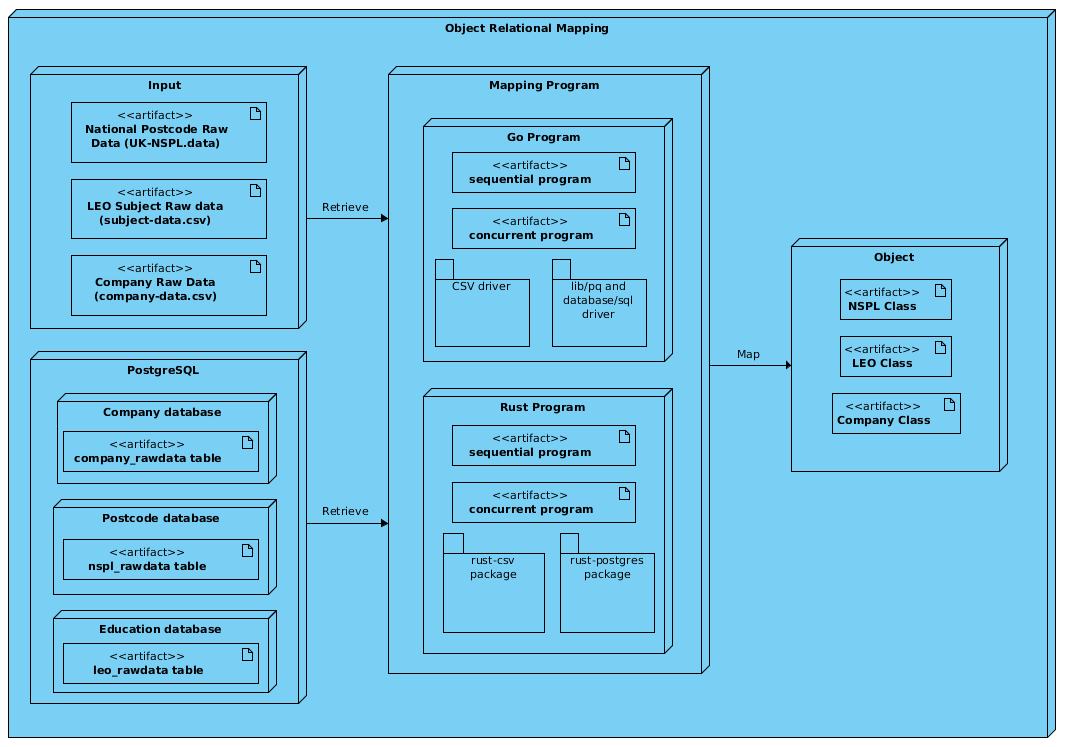
\includegraphics[width=1.0\textwidth]{FYP2/Chapter3/FYP2-ORM-deployment.png}
		\rule{35em}{0.5pt}
	\caption[Data Retrieval with ORM Deployment Diagram]{Data Retrieval with ORM Deployment Diagram}
	\end{figure}


Object-Relational Mapping (ORM) is a technique to manipulate data from database with object-oriented paradigm. The data retrieve from CSV data sources and PostgreSQL database will be convert into object model to ease the manipulation of data in discipline manner. \cite{orm-introduction} The approach increase usability, flexibility and improve data handling for Data Cleaning and Data Migration.

Figure 3.16 shows the ORM deployment diagram that provide graphic representation of mapping between object and data with mapping program written in Go and Rust programming language. In this project, we will construct our own ORM tools tool for data retrieval from CSV file and PostgreSQL database with the assistance of CSV package driver, PostgreSQL driver and built-in SQL library from respective language. 

All the rows of data will be retrieved from PostgreSQL database and CSV file with Go and Rust's ORM to conduct performance comparison between sequential and concurrent execution and concurrent programming languages' expressive power. The results will be recorded and compared. 

\section{Data Cleaning}

\subsection{Introduction}

Data cleaning is the action of detecting and removing missing, incomplete and data redundancy within database. \cite{data-cleaning-definition} The inconsistencies and incorrect records will be detected in the datasets obtained from the secondary sources because we have lack of control over the data quality. 

Data redundancy occurs within a data storage when same piece of data exists in two separate places or two different fields within a single database. Database without normalization will cause updation, deletion and insertion anomalies. The table below is used to understand these the impact of these anomalies on causing data inconsistencies. 

\begin{figure}[H]
	\centering
	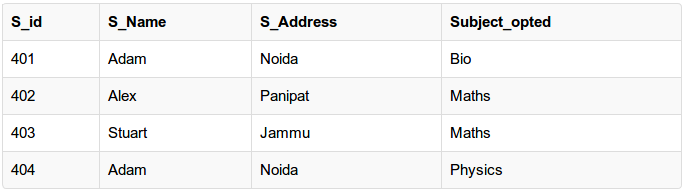
\includegraphics[width=1.0\textwidth]{FYP2/Chapter3/denormalization-example.png}
	\rule{35em}{0.5pt}
	\caption[Student table without normalization]{Student table without normalization}
\end{figure}

\begin{enumerate}[topsep=0pt,itemsep=-1ex,partopsep=1ex,parsep=1.5ex]
	
	\item \textbf{Insertion anomaly.} If student don't enroll any subject and \textbf{subject} is a mandatory field, the records cannot be insert into the database without the presence of other attributes or columns. 
	\item \textbf{Deletion anomaly.} If specific student willing to drop a subject, the entire records are forced to delete. As a result, certain attributes or part of the records are lost due to deletion of specific attributes without awareness which leads to missing data.
	\item \textbf{Updation anomaly.} To update student address in the table, the entire \textbf{address} column are required to be updated. If the duplicate records in the database are partially updated, it will leads to data inconsistency. 
	
\end{enumerate}

Therefore, \textbf{database normalization} and \textbf{data standardization} is conducted to improve the quality and reliability of the datasets.

\subsection{Database Normalization}

\subsubsection{Introduction}

Data normalization is conducted to eliminate data redundancy and improve data integrity. The mentioned method is an approach to remove all the data anomalies and recover the database into consistent state. \cite{normalization-benefits} Normalization is a multi-step approach and require rules to organize data into tabular forms and define relationships among them. The normalization rules and description are listed as follow: 

\begin{enumerate}[topsep=0pt,itemsep=-1ex,partopsep=1ex,parsep=1.5ex]
	
	\item \textbf{First Normal Form (1NF).} The rule required to eliminate repeating groups, identify primary key and discover \textbf{partial dependencies} or \textbf{transitive dependencies} among column by determine the determinant of the records. 
	\item \textbf{Second Normal Form (2NF).} The rule required to create new table with primary key assigned for \textbf{partial dependencies} elimination. 
	\item \textbf{Third Normal Form (3NF).} The rule required to create new table with primary key assigned for transitive dependencies elimination. 
	
\end{enumerate}

Relational database design is conducted to define entities, attributes, relationships and keys to fulfill normalization rules on eliminating data redundancy. The information contains in raw data are divided and separated into specific table and establish relationship among them to form an organized database. Ultimately, naming conventions and standards are used to form table to increase the usability and maintainability of database. 

\subsubsection{Phase 2 Normalized Company Entity Relationship Diagram} 

\begin{figure}[H]
	\centering
	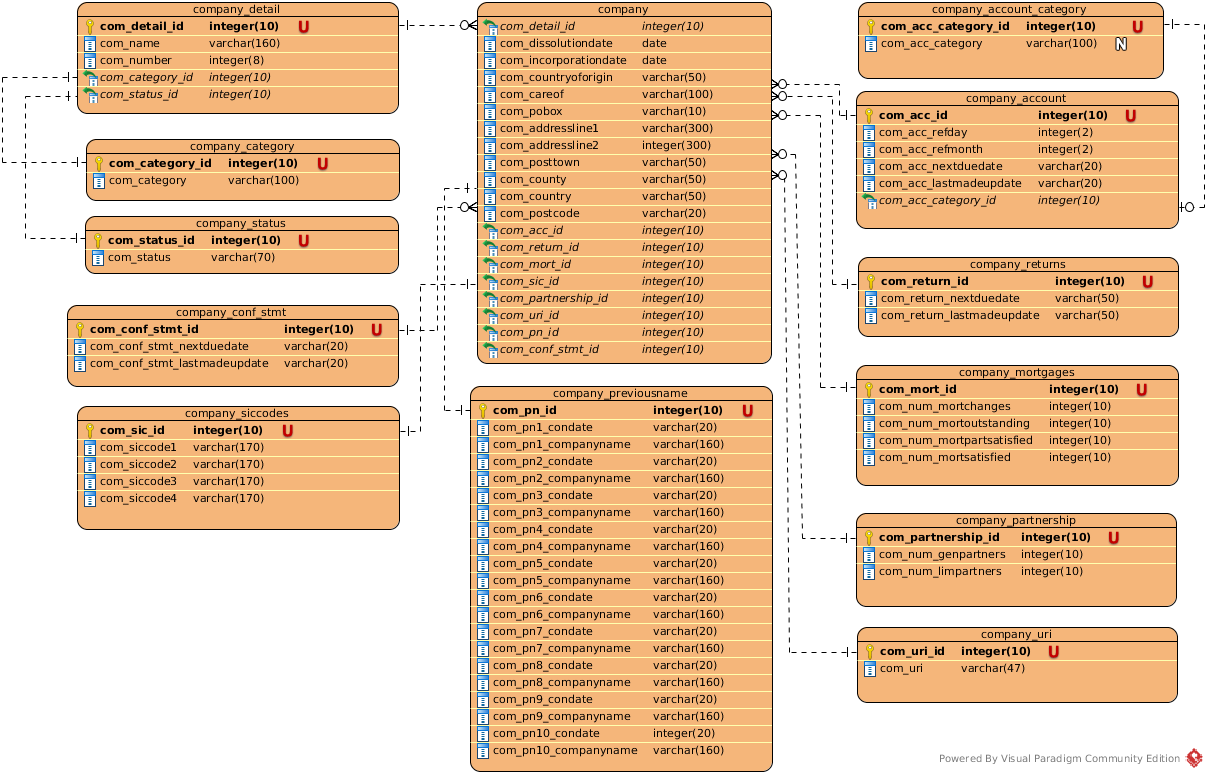
\includegraphics[width=1.0\textwidth]{FYP2/Chapter3/FYP2-Company-Normalized-ERD.png}
	\rule{35em}{0.5pt}
	\caption[Company Normalized Database Design]{Company Normalized Database Design}
\end{figure} 

The figure above shows Company's entity relationship diagram (ERD) to provide a graphical representation of normalized database design that display the relationships of entity stored in a database.

\subsubsection{Phase 2 Normalized Postcode Entity Relationship Diagram}

\begin{figure}[H]
	\centering
	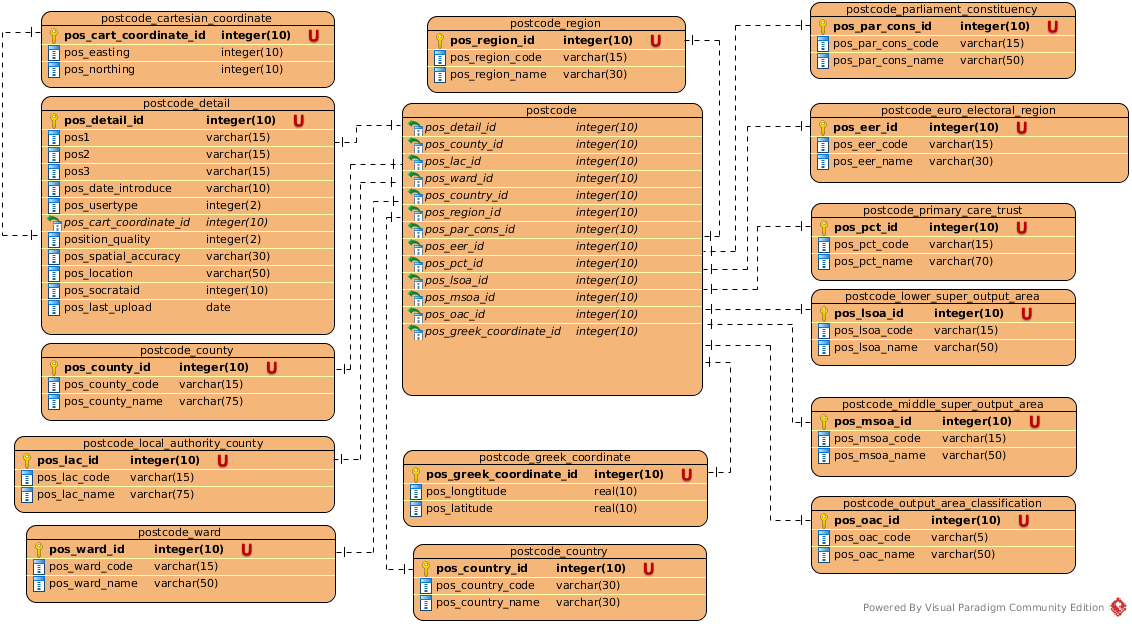
\includegraphics[width=1.0\textwidth]{FYP2/Chapter3/FYP2-Postcode-Normalized-ERD.png}
	\rule{35em}{0.5pt}
	\caption[Postcode Normalized Database Design]{Postcode Normalized Database Design}
\end{figure} 

The figure above shows Postcode's entity relationship diagram (ERD) to provide a graphical representation of normalized database design that display the relationships of entity stored in a database. 

\subsubsection{Phase 2 Normalized Education Entity Relationship Diagram} 

\begin{figure}[H]
	\centering
	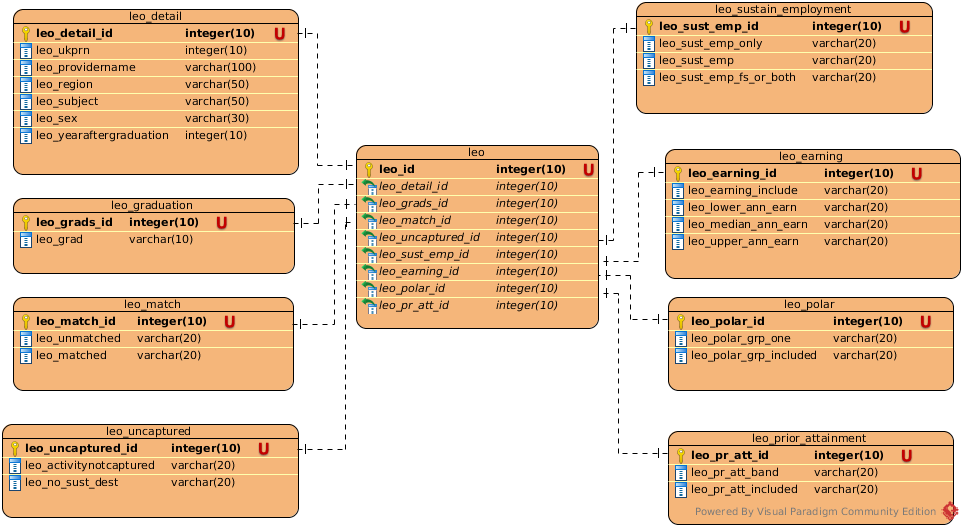
\includegraphics[width=1.0\textwidth]{FYP2/Chapter3/FYP2-Education-Normalized-ERD.png}
	\rule{35em}{0.5pt}
	\caption[Education Normalized Database Design]{Education Normalized Database Design}
\end{figure} 

The figure above shows Education's entity relationship diagram (ERD) to provide a graphical representation of normalized database design that display the relationships of entity stored in a database.

\subsection{Data Cleaning Parser}

\subsubsection{Phase 2 Company Data Cleaning Parser Deployment Diagram}

\begin{figure}[H]
	\centering
	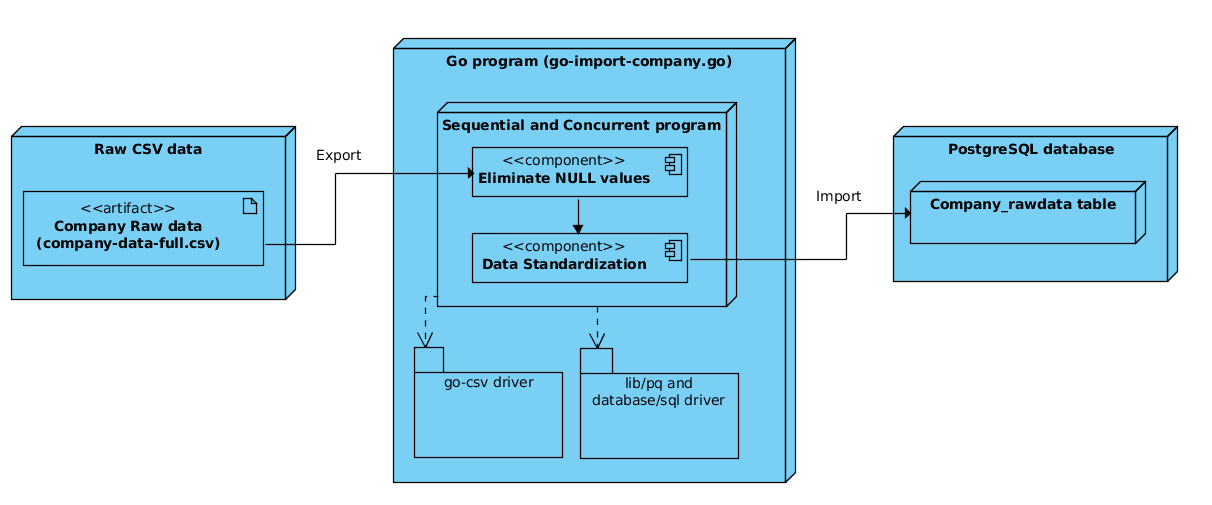
\includegraphics[width=1.0\textwidth]{FYP2/Chapter3/FYP2-data-cleaning-deployment.png}
	\rule{35em}{0.5pt}
	\caption[Company Data Cleaning Parser Deployment Diagram]{Company Data Cleaning Parser Deployment Diagram}
\end{figure} 

The figure 3.18 shows the deployment diagram of company data cleaning parser. 

The cleaning parser is written with Go program language that consume encoded company raw data (performed in Section 3.3) as input and make execution decisions to eliminate NULL values and perform data standardization to repair missing and incorrect data. Afterwards, the cleaned data will be stored into PostgreSQL database await to be processed. The program work similarly as ORM (mentioned in Section 3.5) by utilizing go-csv driver to retrieve data from CSV files and lib/pq or database/sql driver to establish connection and perform transaction with the PostgreSQL database. 

\section{Database Tuning}

\subsection{Phase 2 Database Tuning Flowchart}

\begin{figure}[H]
	\centering
	\includegraphics[width=0.65\textwidth]{FYP2/Chapter3/FYP2-database-tuning-flowchart.png}
	\rule{35em}{0.5pt}
	\caption[Database Tuning Flowchart]{Database Tuning Flowchart}
\end{figure} 

Database tuning is a process of configure PostgreSQL database's environment to optimize performance by increase throughput and decrease response time. The approach required to open PostgreSQL database configuration file with root access in Linux Operating System environment. The configuration made and reason to perform are describe as follow: 

\begin{enumerate}[topsep=0pt,itemsep=-1ex,partopsep=1ex,parsep=1.5ex]
	
	\item \textbf{Max Connection.} The number max connection of PostgreSQL database is modified to allow more \textit{Goroutines} from Go program to establish database connection concurrently and perform parallelize transaction. This modification helps increase performance on Data Cleaning and Data Migration in this project. If the connection pool is not modified, the database system will display FATAL error and terminate the process immediately. 
	\item \textbf{Shared Buffer.} The parameter of shared memory buffer shall be modified as 25 percents of memory in our systems. Increase the amount of memory PostgreSQL database uses for shared memory buffers allow the database to handle extra workloads. 
	\item \textbf{Shared Memory.} The maximum size of shared memory segment shall be modified to allow \textit{Goroutines} or \textit{threads} access to PostgreSQL database simultaneously for better data passing and avoid redundant copies. This configuration parameter determine dedicated memory for PostgreSQL to caching data and increase the space for threads to communicate with the database. The parameter shall be modify with Bytes(B). 
	
\end{enumerate}

Ultimately, restart of PostgreSQL database is required to update the changes and modifications. 

\section{Data Migration} 

Data migration is the process of transferring data within storage system for database migration. \cite{data-migration-definition} Data migration is extremely challenging as we need to take care of performance issues, data integrity, data consistency and prevent data corruption. The data should be protect carefully and prevent missing during the migration process. 

\begin{landscape}
	\subsection{Phase 2 Data Migration Deployment Diagram} 
	\begin{figure}[H]
		\centering
		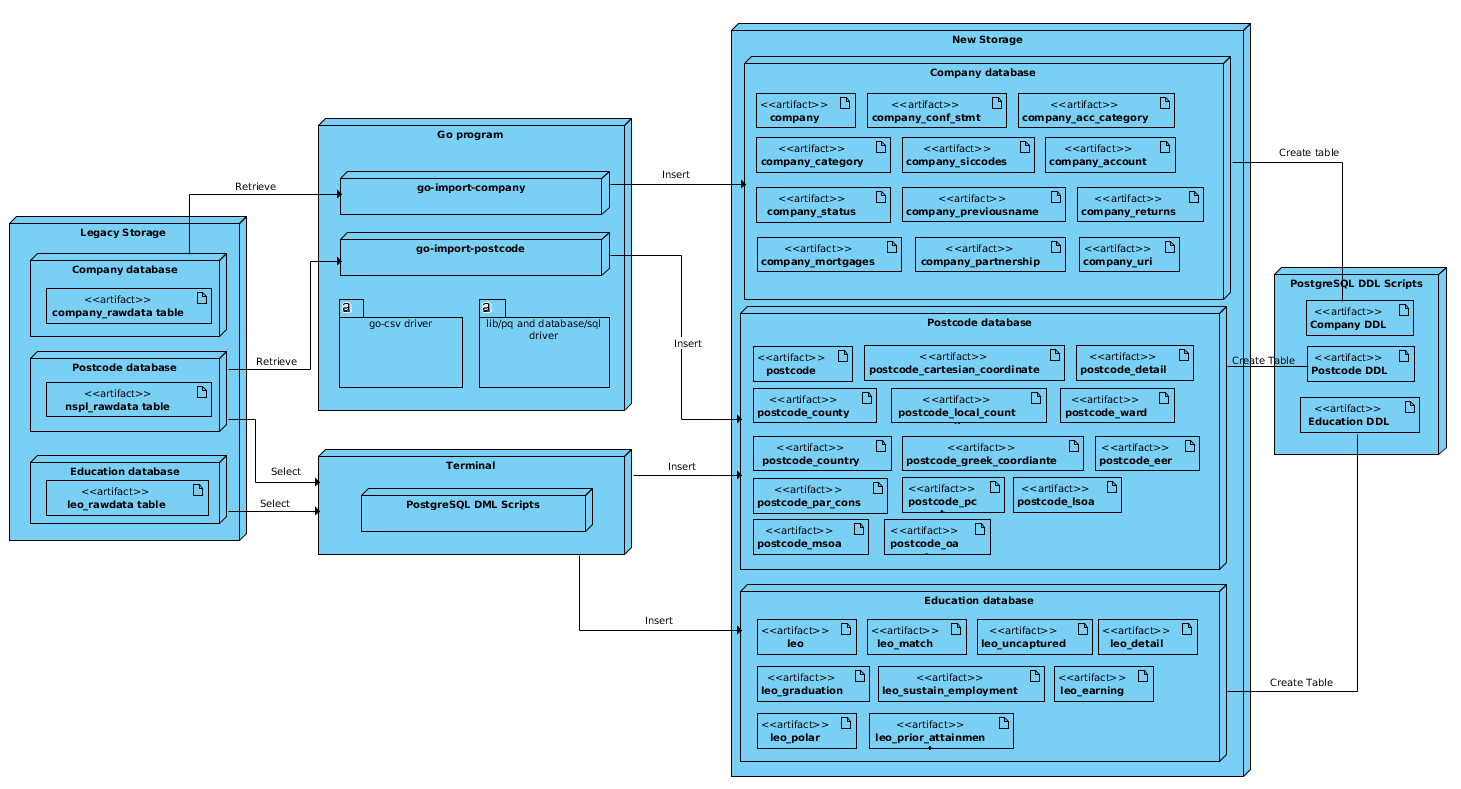
\includegraphics[width=1.4\textwidth]{FYP2/Chapter3/FYP2-data-migration-deployment.png}
		\rule{35em}{0.5pt}
		\caption[Data Migration Deployment Diagram]{Data Migration Deployment Diagram}
	\end{figure}
\end{landscape}

Figure 3.20 shows the deployment diagram of data migration process. 

The normalized table in all database are created with PL/pgSQL DDL scripts. Once the creation of table is successful, the data migration of education database is performed with PL/pgSQL DML script running in terminal environment. The mentioned database is migrated with script because it only contains 30000+ rows and its lightweight to be process with queries. 

Afterwards, the postcode and company database are migrated from legacy storage to new storage with the execution of scripts and Go program as shown in Figure 3.23. Both company and postcode data are migrated with Go program because it contains more than 4 millions rows in total and its difficult to handle with queries. The unique data is extracted from legacy storage and stored into the normalized table in new storage. 

The postcode migration program is developed with \textbf{Channel Synchronization} concepts to perform data migration execution across goroutines to form an concurrent execution. The synchronization primitives of Go programming language is used to perform communication between threads within channel in mutual exclusion locks.

Other than that, the company migration program is developed with \textbf{Semaphore} concepts to apply control access of 400,000 \textit{Goroutines} on common resource provided by PostgreSQL database and operating system environment. The concurrency of data migration execution in this program are controlled and limited to prevent race condition. These Goroutines are required to communicate with each other to utilized 299 open connection with PostgreSQL database on migrating 3.5 millions of data with specific resource provided. 

The migration program is written with Go programming language with the inclusion of database/sql driver to establish connection and lib/pq driver to perform transaction with PostgreSQL database. All the migration process does not modify the source data in legacy storage to serve as backup for in case of emergence. In addition, the changes of migration can be easily tracked for verification purposes. Ultimately, the migration duration is recorded and measured.  


% MAIN SECTION ===============================
%\section{Chapter Summary}
%Your job here
